\chapter{Implementation}

\section{System Architecture}
\label{sec:sys-arch}

\begin{figure}[ht]
    \centering
    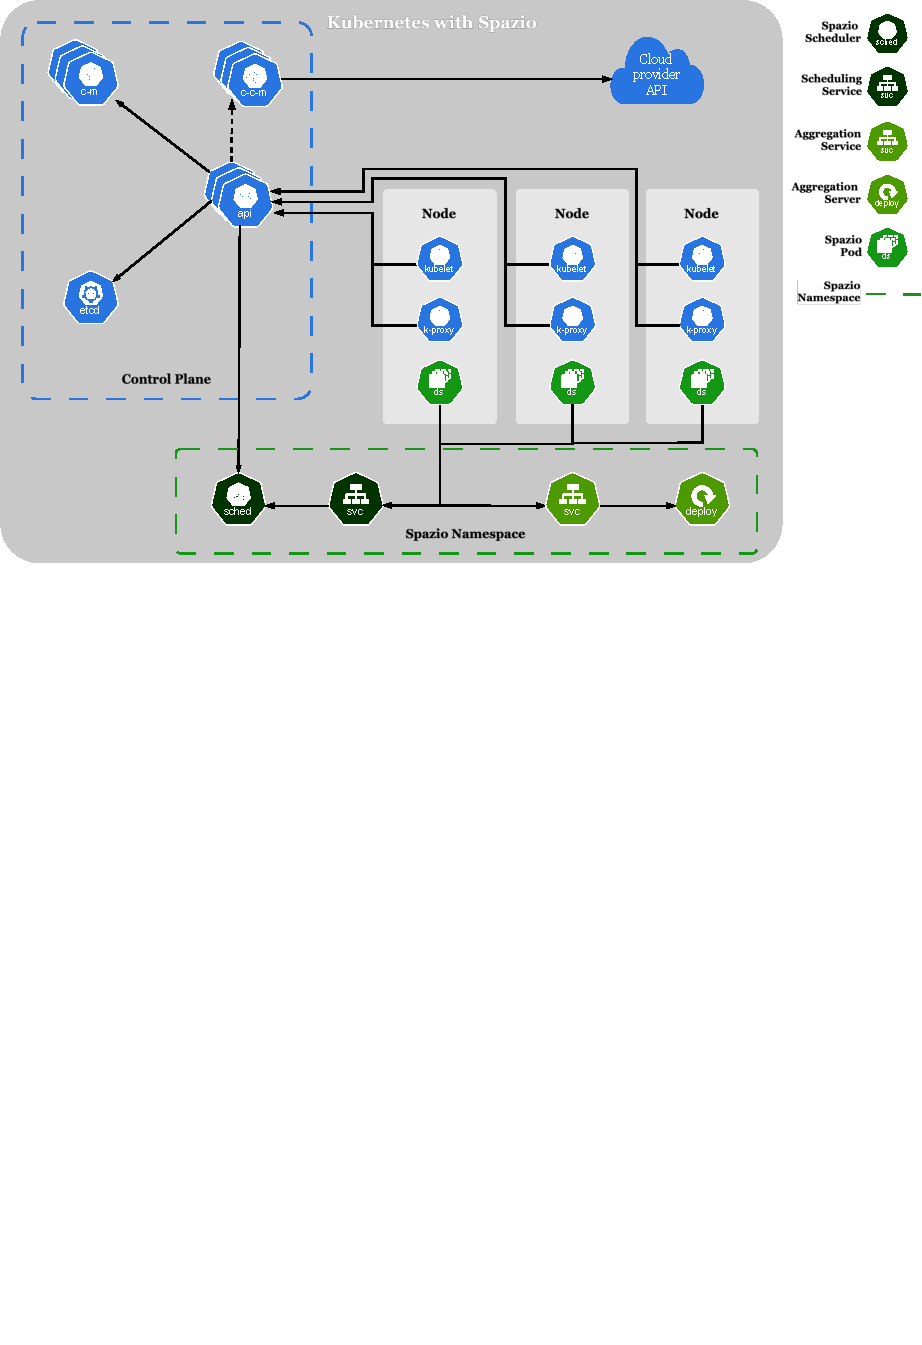
\includegraphics[width=\textwidth]{images/carico-svg.pdf}
    \caption{The components within the \textsc{Carico} system}
    \label{fig:spazio-system}
\end{figure}

The \textsc{Carico} system consists of three core components (shown in figure
\ref{fig:spazio-system}):
\begin{itemize}
    \item \textsc{Carico} DaemonSet: each Node in the cluster will contain a \textsc{Carico} Pod.
        This Pod periodically collects telemetry from the Node and generates its
        local model and a capacity signal, which it sends to the Scheduling
        Service. When the \textsc{Carico} Pod deems its local model outdated, it requests
        the latest aggregated global model from the Aggregation service.
    \item Aggregation Server: This deployment provides the Aggregation service.
        The Aggregation Server Pod receives local models from Nodes
        and returns the latest aggregated global model.
    \item Scheduler: In \textsc{Carico}, the scheduler is a \textbf{Scheduler Plugin},
        implementing custom Filter, Score and Reserve functions. It also acts as
        the server of the Scheduling service, receiving the latest capacity
        scores of each Node to inform its scheduling decisions.
\end{itemize}

\section{\textsc{Carico} Pod}
\begin{figure}[H]
    \centering
    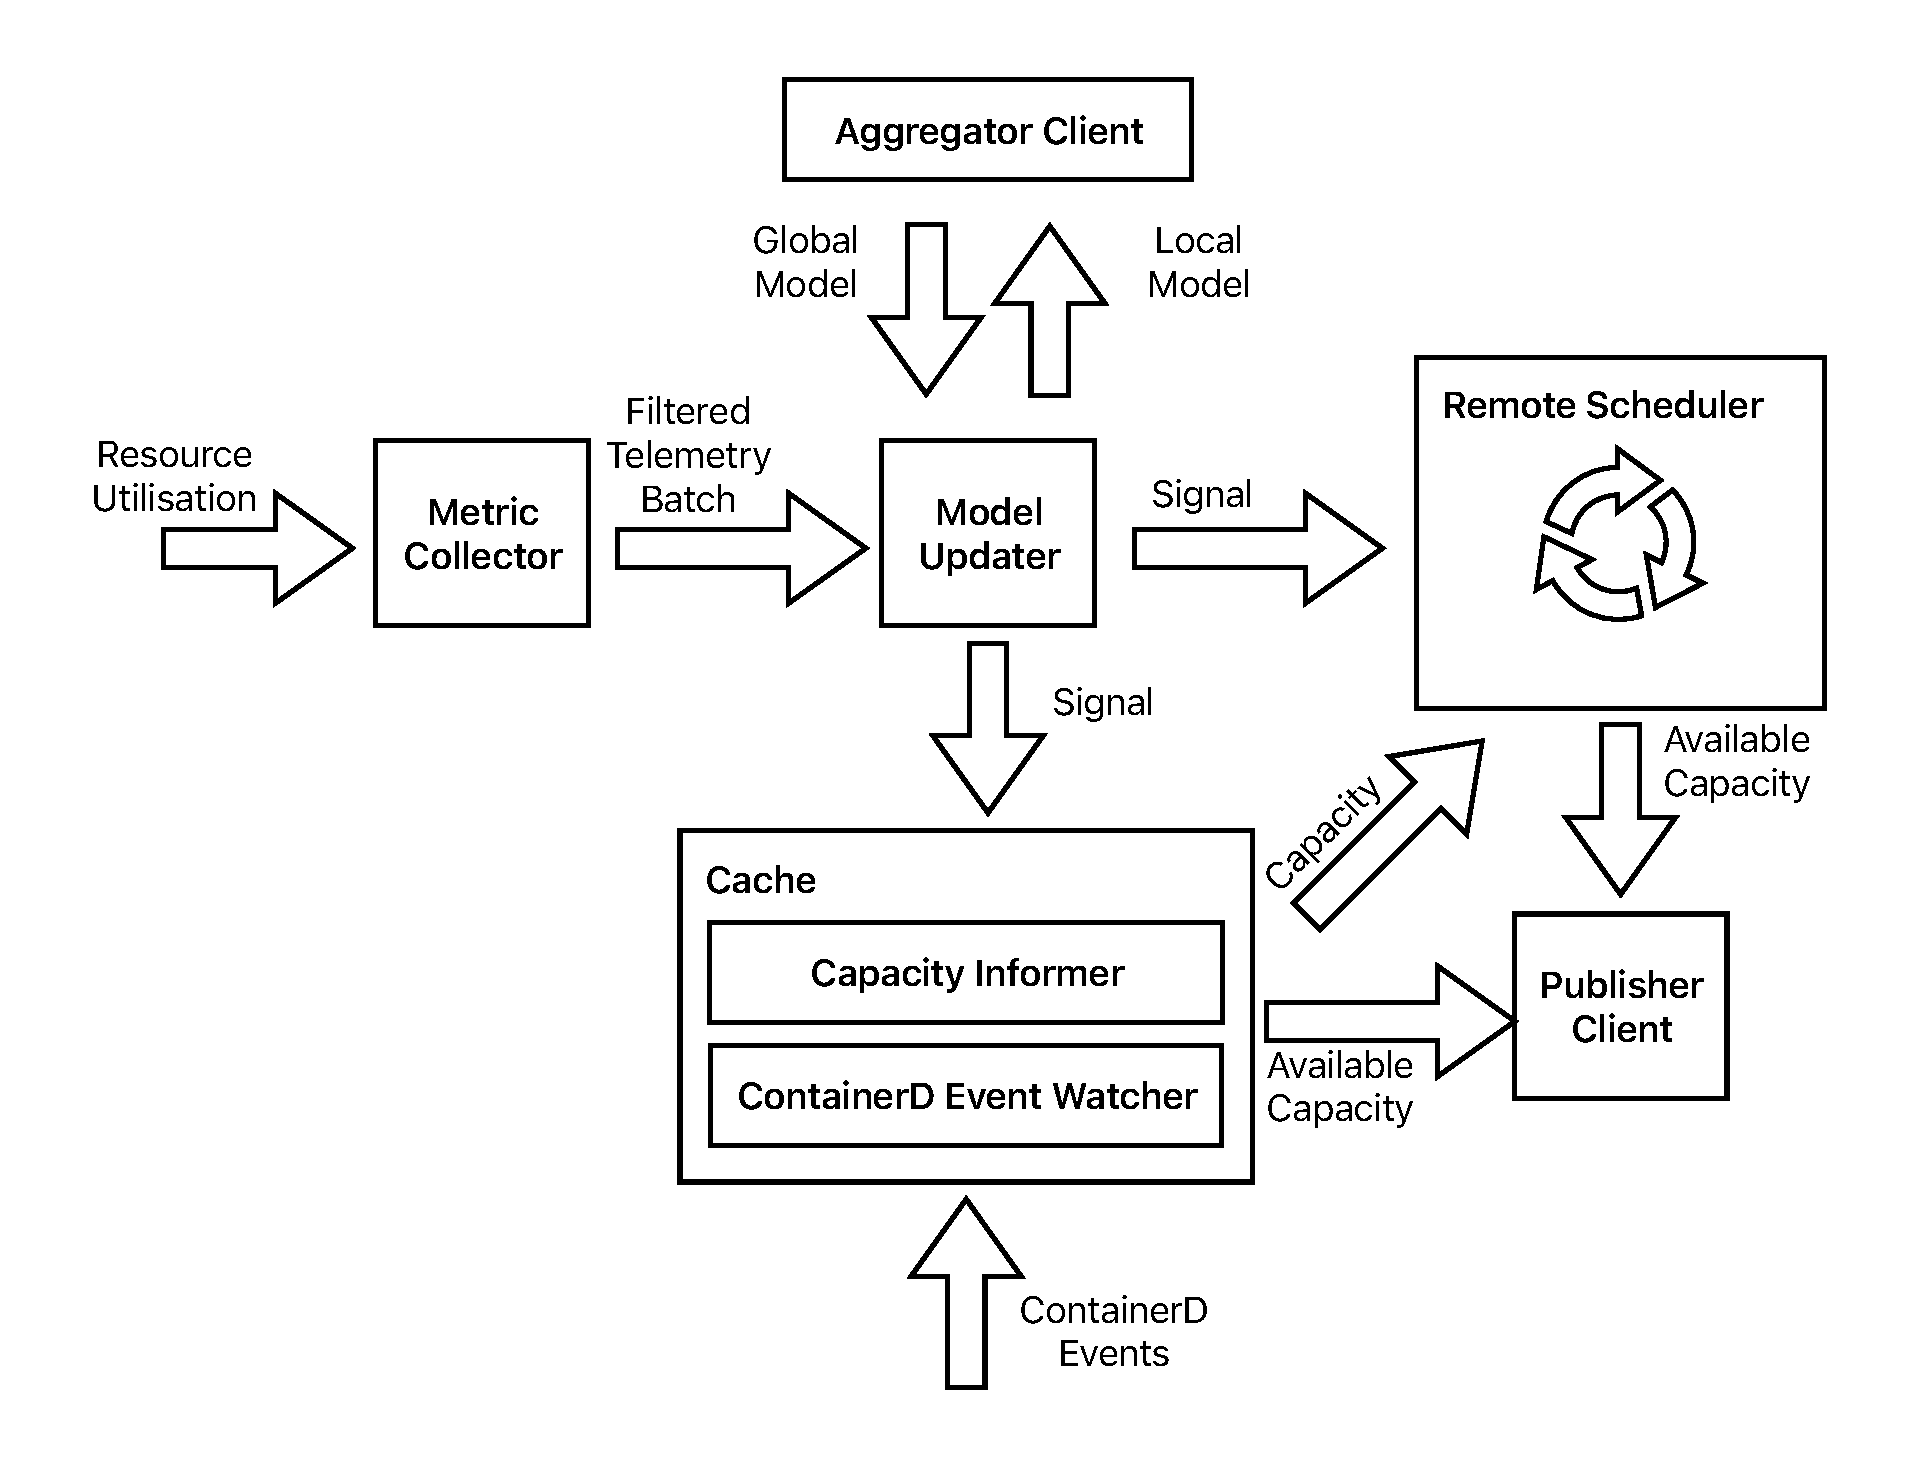
\includegraphics[width=\textwidth]{images/spazio-pod.pdf}
    \caption{Core components within the \textsc{Carico} Pod}
    \label{spazio-pod-components}
\end{figure}
As mentioned in section \ref{sec:sys-arch}, the \textsc{Carico} Pods are defined within a
DaemonSet - a DaemonSet ensures that all Nodes run a copy of a Pod. The \textsc{Carico}
Pods collect telemetry from the Node and generate its local model and capacity
signal. The following sections detail the metrics considered and explain the
corresponding implementation decisions.

\subsection{Metric Collection}
To build its local model, the \textsc{Carico} Pod must first collect telemetry.
Kubernetes offers numerous ways to obtain telemetry data. I explored two primary
sources of telemetry data:
\begin{itemize}
    \item Metrics Server: a cluster add-on that acts as a centralised source of
        container reosurce metrics.
    \item \verb|/proc/|: a pseudo-filesystem within Linux that exposes real-time
        information about running processes and system's hardware.
\end{itemize}

With Metrics Server, a scraper is used to periodically (default every 15
seconds) collects resource metrics from Kubelets and exposes them from its
\verb|metrics.k8s.io/v1| APIService. While simple to use, it offers limited
metrics (CPU and RAM utilisation only) and introduces additional latency.
Moreover, its default 15 seconds scraping interval is too infrequent,
potentially missing short-lived Pods entirely.

\verb|/proc/|, conversely, offers low latency access to an up-to-date view
of the current state of the system. Furthermore, \verb|/proc/| contains various
files and subdirectories, each providing specific information. Examples include,
\verb|/proc/stat| which contains the amount of time CPU cores spend in different
states, \verb|/proc/meminfo| provides statistics about memory usage,
\verb|/proc/diskstats| presents the raw, low-level I/O statistics of all block
devices. Finally, both these sources are not generated periodically, but rather
on-the-fly. This guarantees that the information you see is as current as the
system's internal state.

Given these advantages, I selected \verb|/proc/| as the source of telemetry
data. The subsequent sections detail the metrics I considered and their
rationale behind their use.

% I decided to collect CPU and memory utilisation as my telemetry data, as these
% metrics are easily accessible and are used in a variety of industry-standard
% schedulers
 % In addition, it would take $15 \times \text{batch size}$
% seconds between model updates (required to collect a single
% batch before performing subspace merging), and would result in a less
% representative and out-of-date model of "current" resource usage.

\subsubsection{Utilisation Metrics}
\texttt{/proc/} can generate standard utilisation metrics (e.g., CPU and memory
percentage usage). These metrics are widely used in
industry~\cite{hadoop2016apache,sahasrabudhe_improved_2015}.

To collect CPU utilisation, I used the \verb|/proc/stat| file. This file reports
the cumulative count of "jiffies" (typically hundredths of a second) each CPU
spent in a specific mode \cite{proc_stat5}. I can then calculate CPU utilisation
using:
\[ \text{CPU Usage\%} = 1 - \frac{\Delta\text{idle} +
\Delta\text{iowait}}{\Delta\text{across all fields}} \]
\verb|/proc/meminfo| can also be used to collect memory utilisations. This file
shows a snapshot of the memory usage in kilobytes. The percentage of memory
used can then be calculated from the given field:
\[ \text{Memory Used\%} = 1 - \frac{\text{MemFree} +
\text{Buffers} + \text{Cached}}{\text{MemTotal}}\]

\begin{figure}[H]
    \centering
    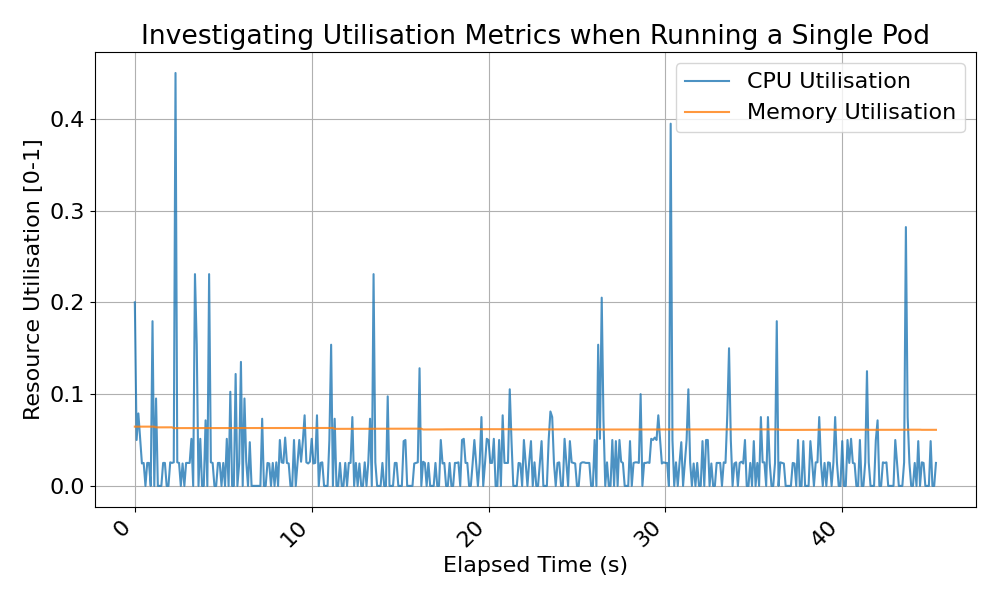
\includegraphics[width=0.45\textwidth]{images/utilisation-baseline.png}
    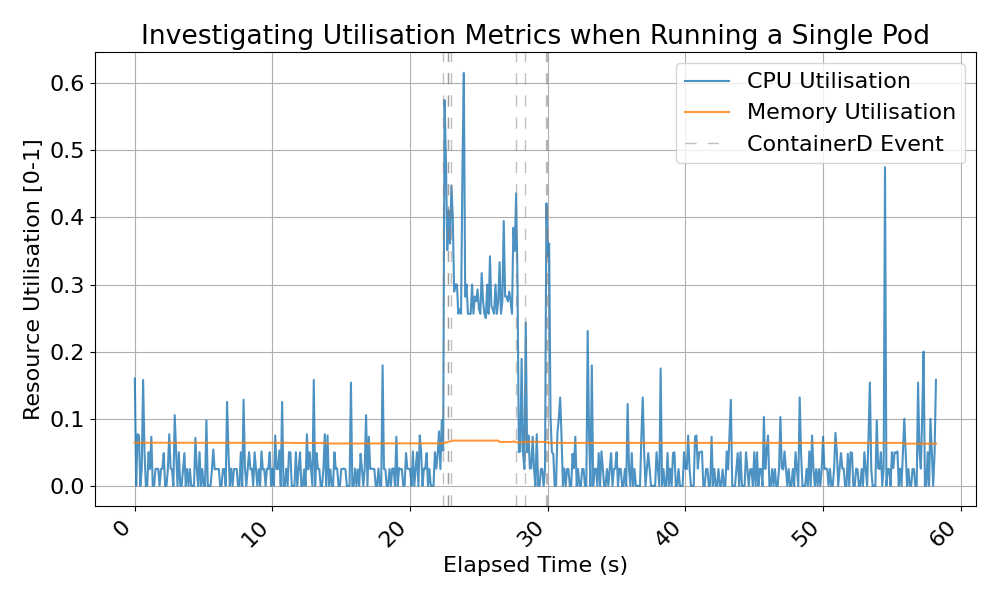
\includegraphics[width=0.45\textwidth]{images/utilisation-single.png} \\
    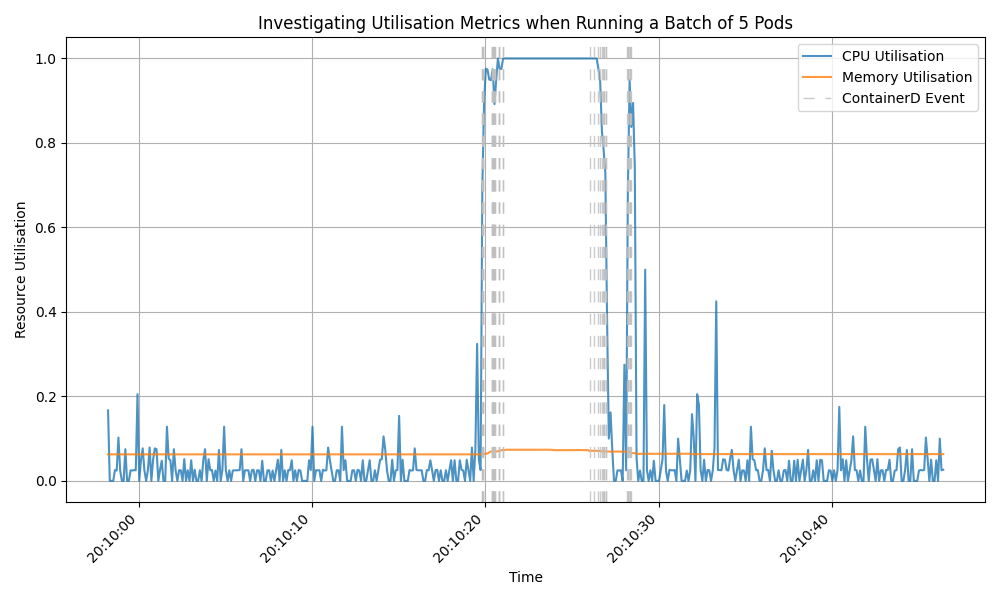
\includegraphics[width=0.45\textwidth]{images/utilisation-smallbatch.png}
    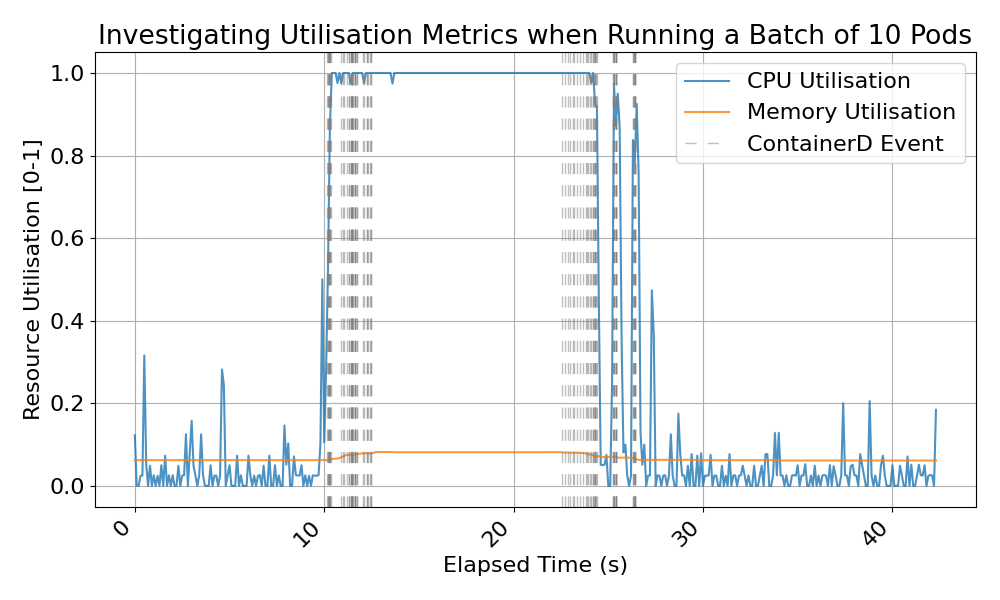
\includegraphics[width=0.45\textwidth]{images/utilisation-bigbatch.png}
    \caption{In this figure we sample CPU and memory utilisation from
    values of \texttt{/proc/stat}, \texttt{/proc/meminfo} at 10Hz during various
    Kubernetes workloads.}
    \label{fig:utilisation-eval}
\end{figure}

To assess their suitability for \textsc{Carico}, I measured utilisation metrics
under various workloads. Figure \ref{fig:utilisation-eval} presents the metrics
behaviour when running different Job sizes of \verb|pi-2000| Pods. For a
CPU-intense workload (calculating $\pi$ to 2000 digits), the CPU utilisation
correctly increased while memory utilisation remained stable.

\subsubsection{Issues of using CPU Utilisation}
\label{sec:issue-with-util}
Early prototypes using only utilisation metrics showed poor throughput compared
to the default \verb|kube-scheduler|, highlighting a problem with relying solely
on CPU utilisation. When deploying 1000 Pods, each requesting 100 milliseconds
of CPU time, across 19 Nodes, the \verb|kube-scheduler| would immediately
allocate all Pods evenly across the Nodes. This would result in $\approx$ 45
Pods running on each Node. In contrast, \textsc{Carico} (using only utilisation
telemetry) allocated at most 5 Pods concurrently per Node. In both situations,
CPU utilisation was 100\%, however, the default \verb|kube-scheduler| managed to
achieve a high throughput, even with a long-tailed distribution of individual
Pod completion times.

\begin{figure}[H]
    \centering
    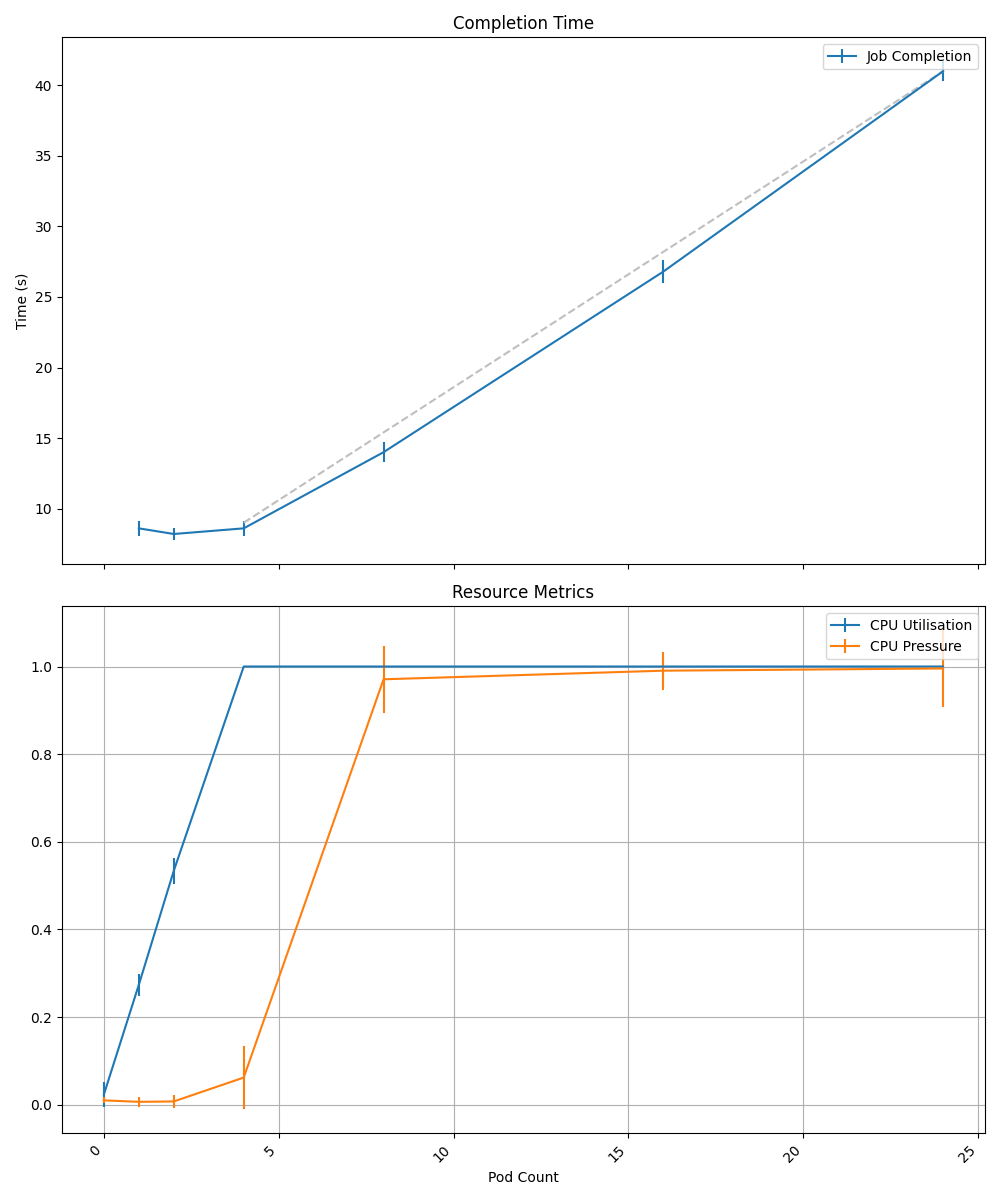
\includegraphics[width=0.45\textwidth]{images/podcount-util-pressure.png}
    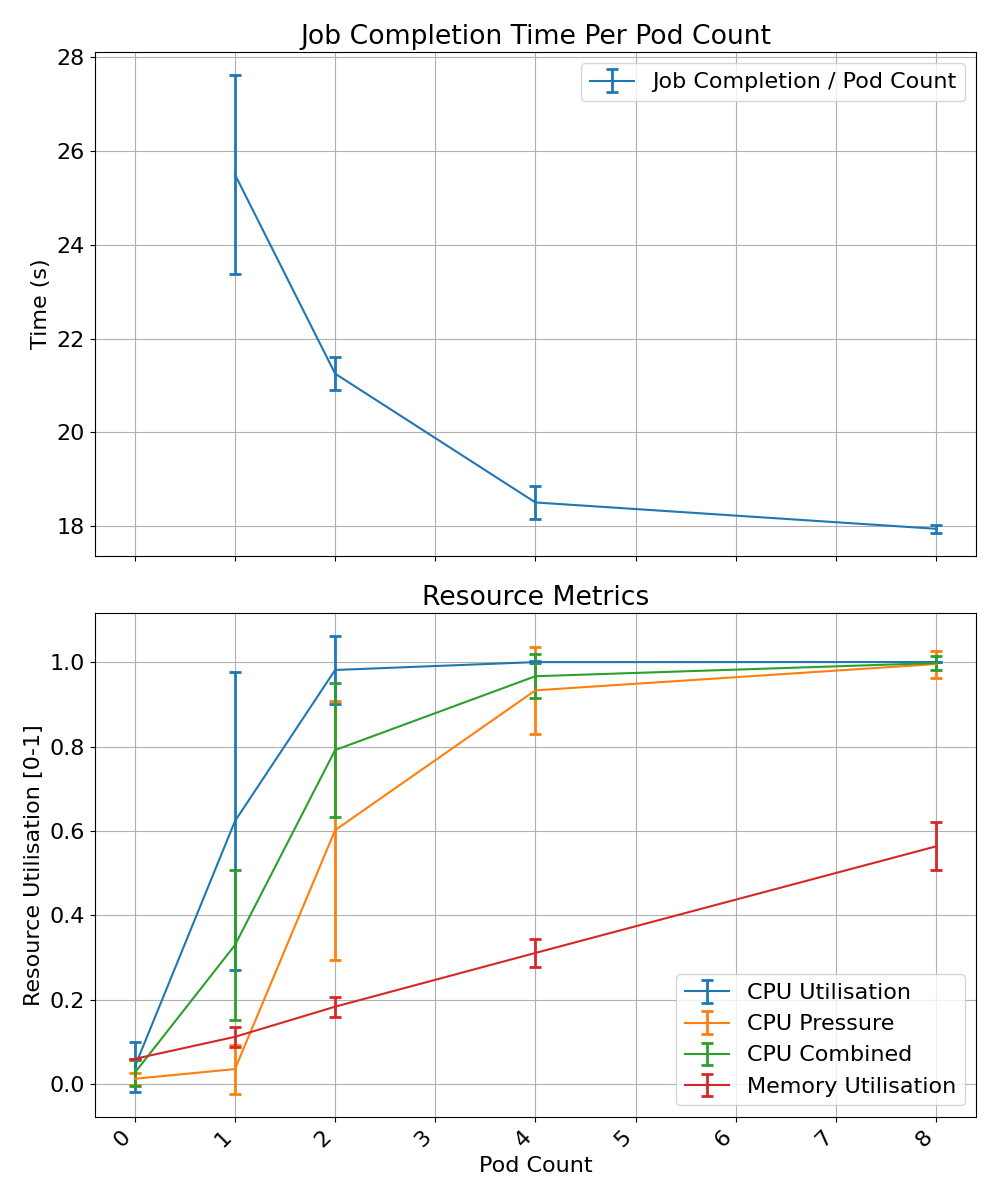
\includegraphics[width=0.45\textwidth]{images/ml-podcount-util-pressure.png}
    \caption{In this figure we sample CPU and memory utilisation from
    values of \texttt{/proc/stat}, \texttt{/proc/meminfo} at 10Hz during various Kubernetes workload.}
    \label{fig:podcount-util-pressure}
\end{figure}

As a result, I decided to further investigate this phenomenon. Figure
\ref{fig:podcount-util-pressure} shows how a Job's completion time changes as you
increase its completion and parallelism count when running different Pods:
cpu-intense Pi-2000 and a small ML workload (training and inference). I also
decided to include measurements from \verb|/proc/pressure|. This investigation
revealed that the relationship between the number of Pods running on
a Node at a time and their completion time showed a close-to linear
relationship. I hypothesise that this is becuase the cluster runs on virtual
machines (VMs). Hypervisors, while abstracting hardware, can mask effects like
cache contention and CPU thrashing. This means that high  CPU utilisation may
not truly signify performance degradation. Thus, CPU utilisation alone is not a
definitive capacity measure, explaining the prototype's initial throughput
limitations.

\subsubsection{Combining CPU Utilisation and CPU Pressure}
Raw \verb|/proc/pressure| metrics were also insuffice as these metrics
barely increased until the Pod count exceeded core count. This would lead to
unreasonably low intial Per-Pod-Cost estimations and an inflated advertised Node
Pod-Capacity. I therefore combined both CPU utilisation and CPU pressure
into a single metric:
\[ CPU = \frac{\text{CPU Utilisation} + \text{CPU Pressure}}{2} \]

This ensures the metric increases with Pod count but doesn't saturate to
quickly. This combined CPU metric only reaches its maximum when \verb|/proc/pressure|
indicates persistant CPU demand (at least one thread always waiting).

\begin{figure}[H]
    \centering
    
\includegraphics[width=0.45\textwidth]{images/blank.pdf}
    \caption{In this figure we investigate the behaviour of combining both CPU
    Utilisation and CPU Pressure.}
    \label{fig:combine-cpu-pressure}
\end{figure}

\subsection{Filtering Metrics}
\textsc{Carico} does not perform peak detection, but its signal is still
susceptible to short-lived spikes. As previously noted,  Pod creation and
deletion incur visible resource usage spikes. These spikes introduce noise
into both the Node's local model, as well as, its Capacity signal. A noisy
signal complicates baseline Capacity and Per-Pod-Cost estimation. As such, I
needed to de-noise the original metrics.

Investigation into the recorded telemetry showed that the spikes caused from
container events would last $\approx$200 milliseconds. Sampling at
10Hz, Dynamic EMA was used to suppress container-event caused spikes (typically
$\approx$ 200ms) while allowing rapid convergence for sustained changes (spikes
$>$ 300ms).

\begin{figure}[H]
    \centering
    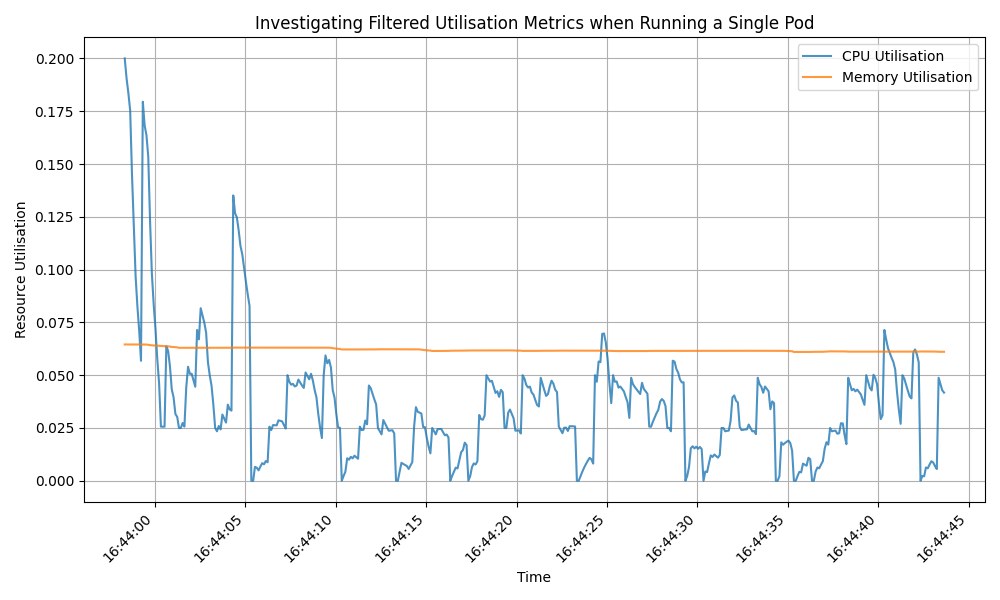
\includegraphics[width=0.45\textwidth]{images/filter-utilisation-baseline.png}
    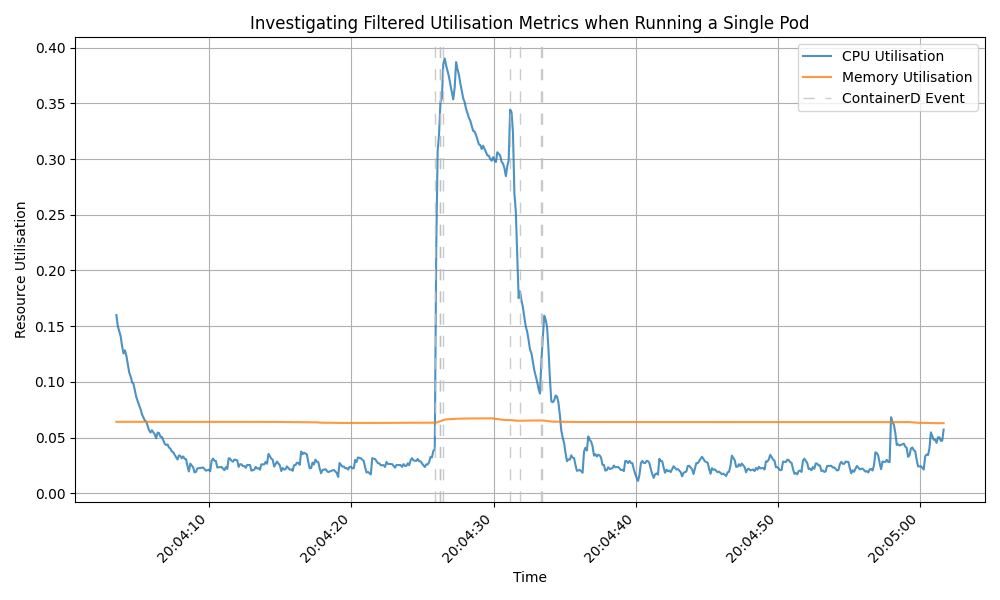
\includegraphics[width=0.45\textwidth]{images/filter-utilisation-single.png} \\
    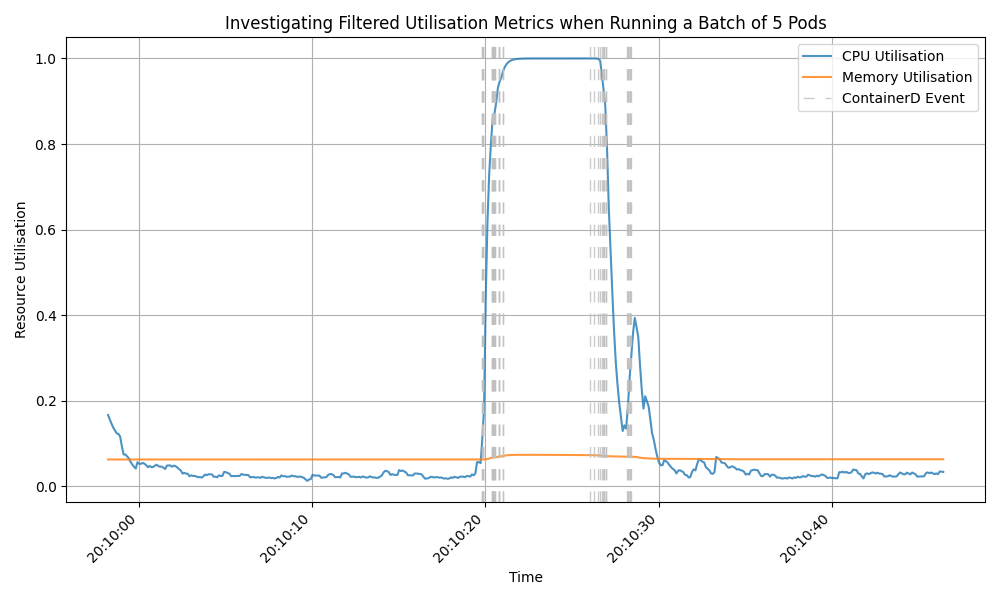
\includegraphics[width=0.45\textwidth]{images/filter-utilisation-smallbatch.png}
    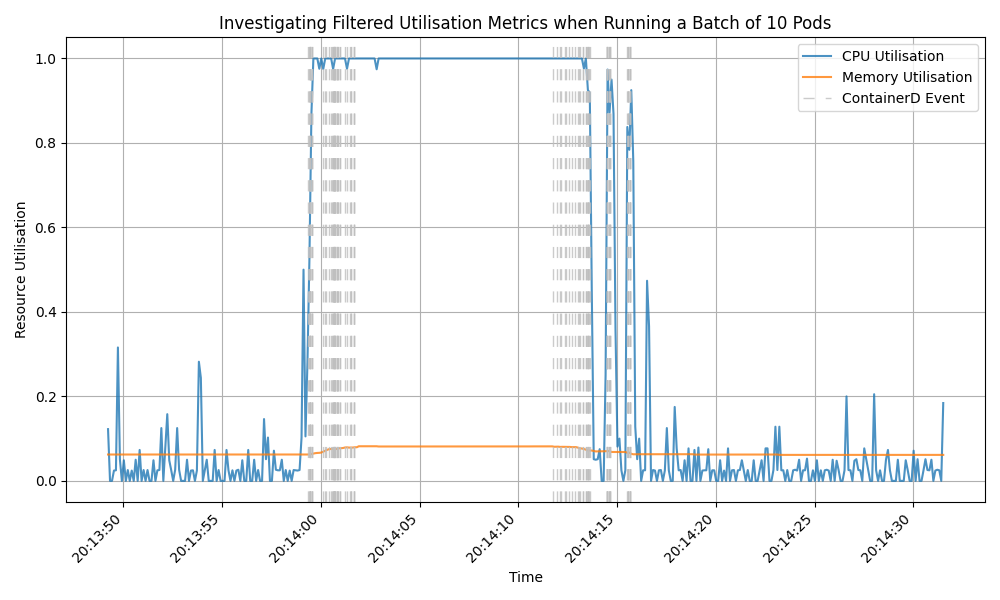
\includegraphics[width=0.45\textwidth]{images/filter-utilisation-bigbatch.png}
    \caption{This figure shows the smoothed metrics under different workloads.}
    \label{fig:filtered-metrics-eval}
\end{figure}

Comparing Figure \ref{fig:utilisation-eval} with \ref{fig:filtered-metrics-eval}
demonstrates the dampening of the Dynamic EMA and its quick responsive to
prolonged changes in workloads. More sophisticated filters were avoided due to
their higher computational cost, which would rob resources from scheduled Pods.
Filtering the signal directly, rather than the telemetry, was considered but
rejected as it would still allow container-event resource spikes to pollute the
local model.

\subsection{Signal Generation}
The \textsc{Carico} Pod calculates its Capacity signal at 1Hz. This matches the local
model update frequency, ensuring that the Capacity signal tracks with the local
model. While a higher frequency would provide the central scheduler a more
current view of a Node's resource status, it would also increase resource
overhead. This overhead would reduce the available resources to other
Pods and could also lower the baseline Capacity signal, potentially reducing
the capacity a Node advertises.

To verify Capacity signal's implementation, I tested it under the scenarios
described in Section \ref{sec:signal-example-scenario}. For the conflicting
workload, I had the measured Node execute a light CPU-focused workload
(\texttt{ng-stress --cpu=8 --cpu-load=25}) with the surrounding Nodes executing
a CPU-intense workload (\texttt{bpi(2000)}). For the complementary workload, the
measured Node executed a light Memory-focused workload (\texttt{ng-stress --vm=4
--vm-bytes=4G}) with the surrounding Nodes also executing the same CPU-intense
workload as in the conflicting scenario. The measured signals are shown in
figures \ref{fig:signal-evaluation-cpu} and \ref{fig:signal-evaluation-mem}

\begin{figure}[H]
    \centering
    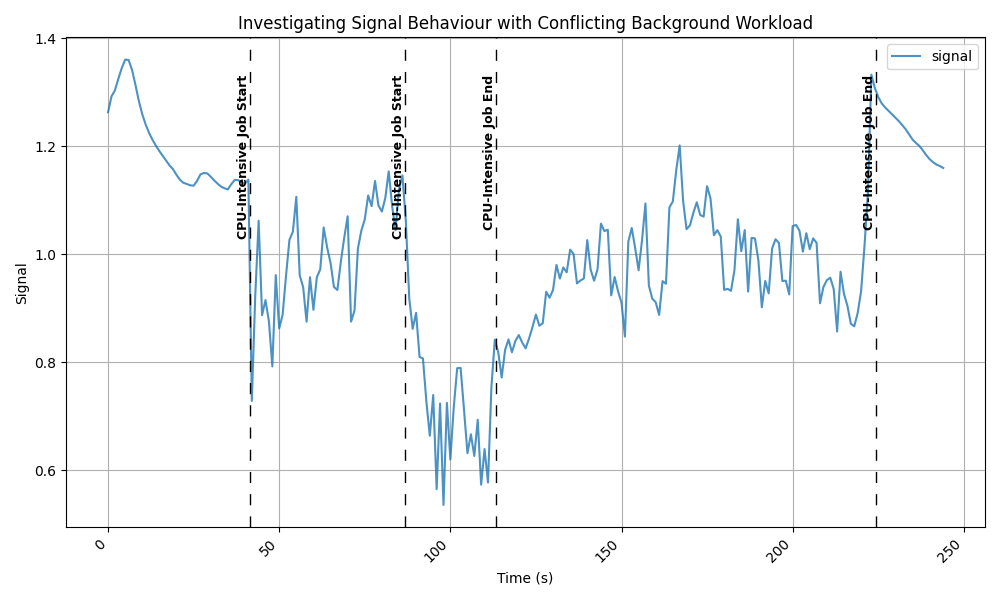
\includegraphics[width=\textwidth]{images/signal-with-cpu.png}
    \caption{The calculated capacity signal of a Node running \texttt{ng-stress
    --cpu=8 --cpu-load=25}. While running this workload, $1000$ Pods running
    \texttt{bpi(2000)} were scheduled across surrounding Nodes.}
    \label{fig:signal-evaluation-cpu}
\end{figure}
\begin{figure}[H]
    \centering
    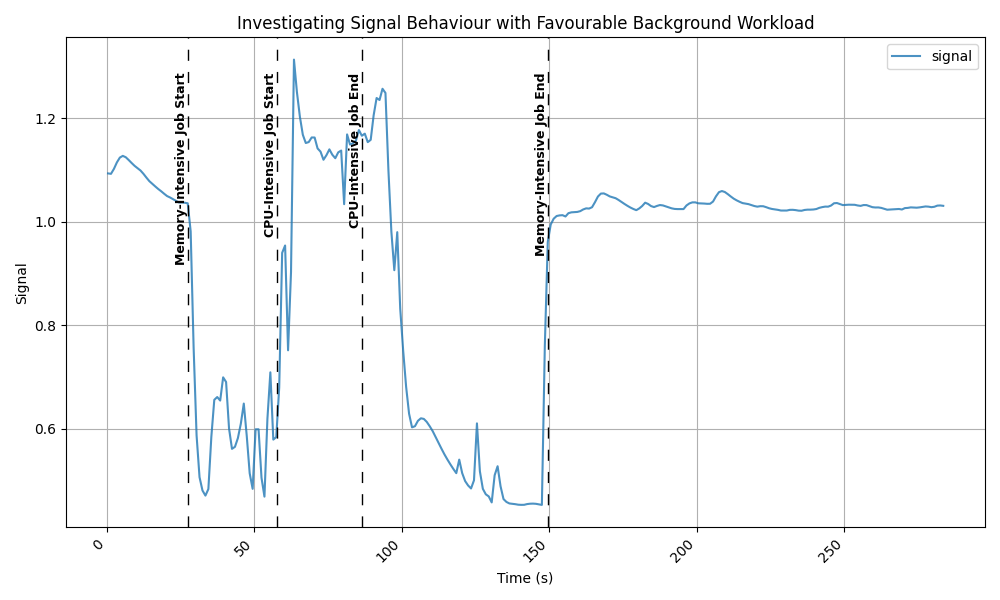
\includegraphics[width=\textwidth]{images/signal-with-memory.png}
    \caption{The calculated capacity signal of a Node running \texttt{ng-stress
    --vm=4 --vm-bytes=4G}. While running this workload, $1000$ Pods running
    \texttt{bpi(2000)} was scheduled across surrounding Nodes.}
    \label{fig:signal-evaluation-mem}
\end{figure}

Figures \ref{fig:signal-evaluation-cpu} and \ref{fig:signal-evaluation-mem}
demonstrates how a Node's capacity signal reacts to changes in surrounding
workloads when experiencing different resource usage. In Figure
\ref{fig:signal-evaluation-cpu}, the measured Node is running a light CPU-focused
workload. Once the CPU-intense workload is scheduled on surrounding Nodes, the
measured Node's capacity signal drops. This is expected as the local models of
surrounding Nodes will reflect a more costly CPU-focused workload. As a result,
when the measured Node aggregates its local model, its new model will reflect
this higher CPU usage with a larger $\sigma_1$ value. Since both the Node's
current resource usageand the learned expected workload (reflected in $u_1$) are
CPU-focused, the increased magnitdue of the expected workload (larger
$\sigma_1$) results in a smaller $k$ (fewer units of this workload can be
added), and thus a lower Capacity signal.

In Figure \ref{fig:signal-evaluation-mem}, the measured Node runs a light
memory-focused workload. When the CPU-intense workload is scheduled on surrounding
Nodes, the measured Node's capacity signal increases. This aligns with the
hypothesis from Section \ref{sec:capacity-signal}. Like in the previous scenario, the global model
reflects a heavy CPU-focused workload, and thus, so will the aggregated local
model of the measured Node. However, with the Node's current resource usage
(memory-focused) now largely orthogonal to the learned expected workload
(CPU-focused), a larger $k$ is required to reach a resource limit.

\subsection{Calculating Cost and Capacity}
Since the \textsc{Carico} Capacity signal incorporates current resource usage,
newly scheduling (but not yet running) Pods do not immediately affect the
Capacity signal. Therefore, a signal reservation mechanism is needed to prevent
the scheduler from greedily overloading the Node with the current highest score.
To handle varyinh Pod workloads, a dynamic estimation of a Pod's "signal cost"
was required. The method also needed to handle concurrent Pod creation and
deletions.

\subsubsection{Detecting Pod Events}
\label{sec:listeners-comparison}
There are numerous ways to detect the addition and removal of Pods from a Node.
I investigated two event detection approaches: watching the Kubernetes API vs
ContainerD events. The goals of the listeners were as follows:
\begin{itemize}
    \item Detect the creation and deletion of Pods to establish a Pod count
    \item Provide warning for potential container-caused churn
\end{itemize}
This warning is crucial because the Dynamic EMA can't fully smooth prolonged
resource spikes from multiple, concurrent container events. Early detection
allows temporarily halting estimations during such bursts.
\begin{figure}[H]
    \centering
    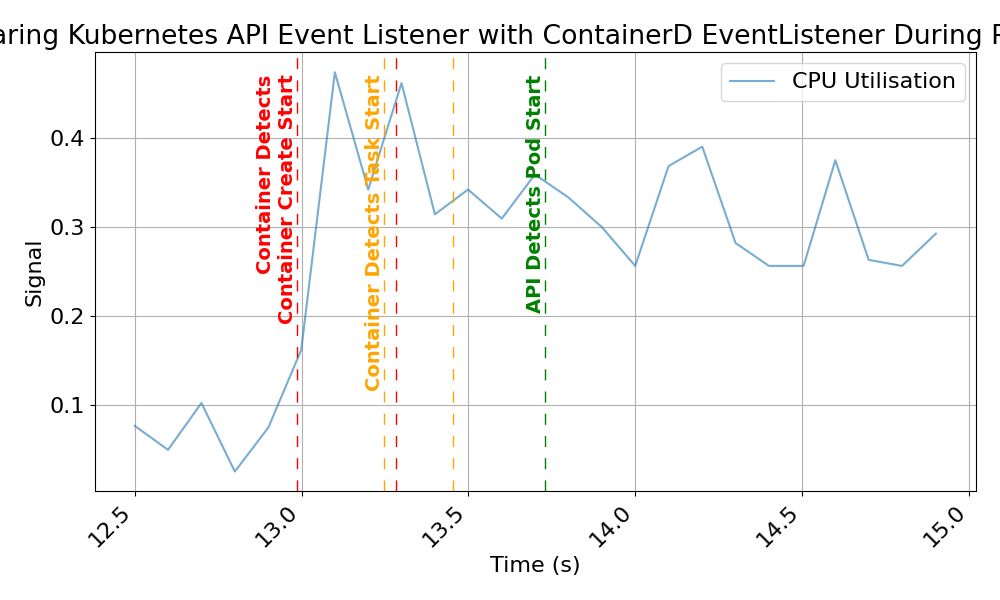
\includegraphics[width=\textwidth]{images/event-comparison-start.png}
    \caption{When different event listeners detected the creation of a Pod.}
    \label{fig:event-evaluation-start}
\end{figure}

\begin{figure}[H]
    \centering
    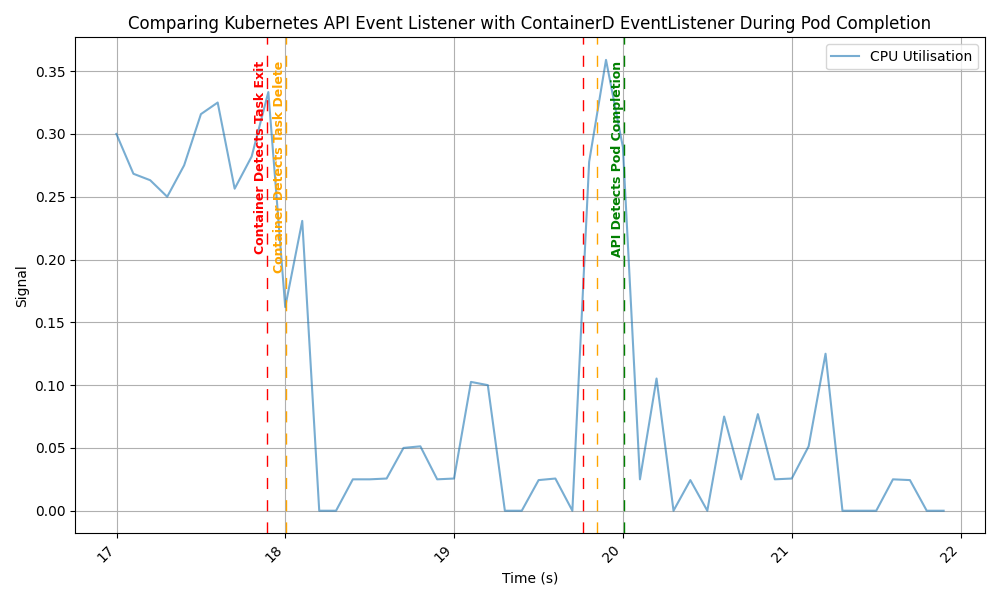
\includegraphics[width=\textwidth]{images/event-comparison-end.png}
    \caption{When different event listeners detected the completion of a Pod.}
    \label{fig:event-evaluation-end}
\end{figure}

Figures \ref{fig:event-evaluation-start} and
\ref{fig:event-evaluation-end} show that communication latency from the
Kubernetes API causes its listener to miss container runtime resource spikes.
Without forewarning, Nodes would incorporate these spikes into
their predictions. On the other hand, we can see that certain container
events precede the spikes. Though more complex, handling ContainerD events
directly provides earlier warnings, reducing noise in calculations.

\subsubsection{Estimating Pod-Cost}
\label{sec:estimating-cost}
To produce a \textbf{reservable} signal, as per Section
\ref{sec:spazio-cost-capacity}, \textsc{Carico} requires Nodes to estimate their
bsaeline Capacity and Per-Pod-Cost. has the capability of estimating its
capacity and per-Pod cost. I needed a streaming signal processing technique with
a low-overhead and the ability to work with a dynamic system (handle changes in
workloads over time). A Kalman filter \cite{} is a powerful algorithm used for
estimating the true state of a dynamic from a series of noisy and uncertain
measurements. It's widely applied in fields like navigation (GPS), robotics,
signal processing and control systems. Its ability to estimate a system's state
from noisy measurements makes it suitable for this dynamic environment.

I devised three Kalman filter-based approaches to estimating reservation costs.
\begin{itemize}
    \item 1D Kalman Filter predicting reservation cost based on the function:
        \[\Delta \text{signal} = \Delta \text{no. of running Pods} \times
        \text{cost}\]
    \item 2D Kalman Filter to predict the signal based on the function:
        \[\text{signal} = \text{capacity} + \text{per Pod cost} \times \text{no.
        of Pods}\]
    \item Two separate 1D Kalman Filters predicting the equation:
        \[\text{signal} = \text{capacity} + \text{per Pod cost} \times \text{no.
        of Pods}\].
        Here, each filter learns a separate variable. This separation prevents
        non-zero covariance entries in the state covariance matrix ($\mathbf{P}$),
        mitigating oscillations observed with a single 2D Kalman filter.
\end{itemize}
To smooth out predictions, I employed two techniques. First, upon detecting
container churn via the event listener, the \textsc{Carico} Pod temporarily
halts estimations. Second, estimations are halted if the Capacity signal reaches
zero. When the capacity signal is 0, it indicates that at least one resource is
at capacity. If this occurs and another Pod begins running on the same Node, the
signal still outputs 0. Otherwise, the filters might inaccurately decrease the
Per-Pod-Cost, leading to an inflated advertised capacity.

\begin{figure}[H]
    \centering
    % 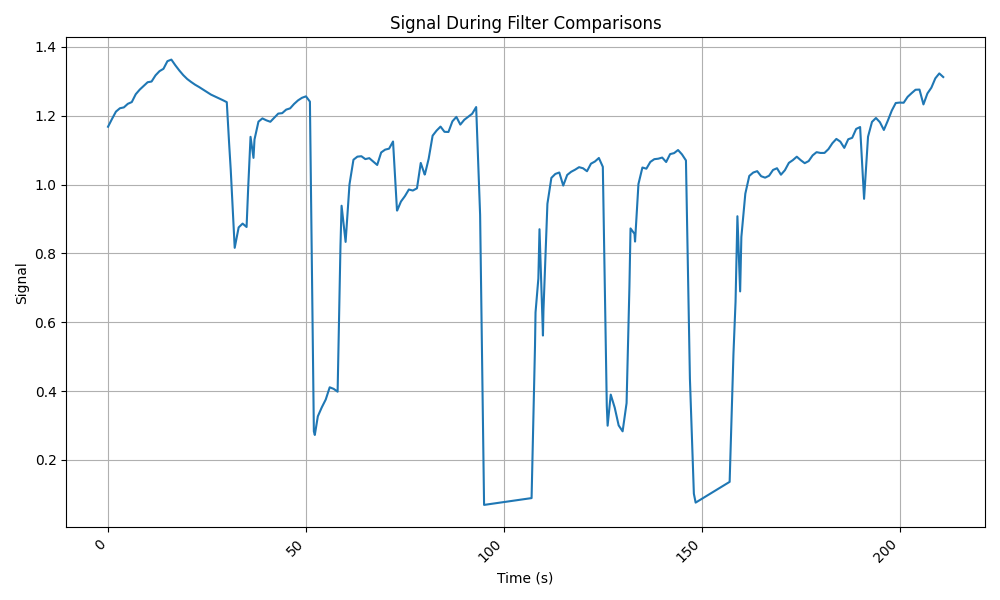
\includegraphics[width=0.45\textwidth]{images/filter-signal.png}
    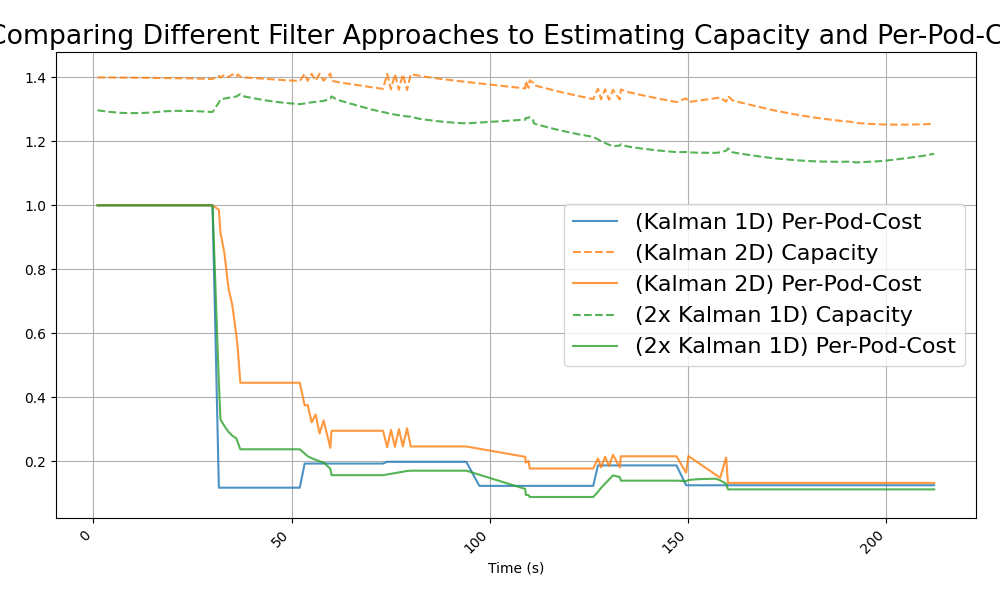
\includegraphics[width=\textwidth]{images/filter-comparison.png}
    \caption{The estimates of the Kalman filters when Node experiences
    variable-sized bursts of \texttt{bpi(2000)} Pods.}
    \label{fig:filter-evaluation}
\end{figure}
To decide the optimal approach, I observed each methods' behaviour when
executing Jobs of various sizes. This is depicted in Figure
\ref{fig:filter-evaluation}.
The $\Delta$-based Kalman filter accurately estimated Per-Pod-Cost, but being
one-dimensional, could not estimate the Node's baseline Capacity signal. The 2D
Kalman filter approach provides a simple method for estimating both the Node's
capacity and its per-Pod cost. Faster convergence for the 2D filter was
attempted using large process noise covariance ($\mathbf{Q}$) values. This, however,
led to large oscillations, as the filter adjusted both baseline capacity and
cost variables to correct errors. The dual 1D Kalman filter was inspired by the
stability of the 1D Kalman filter. This filter converged quickly and accurately
without exhibiting the oscillations that plagued the 2D Kalman filter.

\section{Aggregation Server}
\begin{figure}[H]
    \centering
    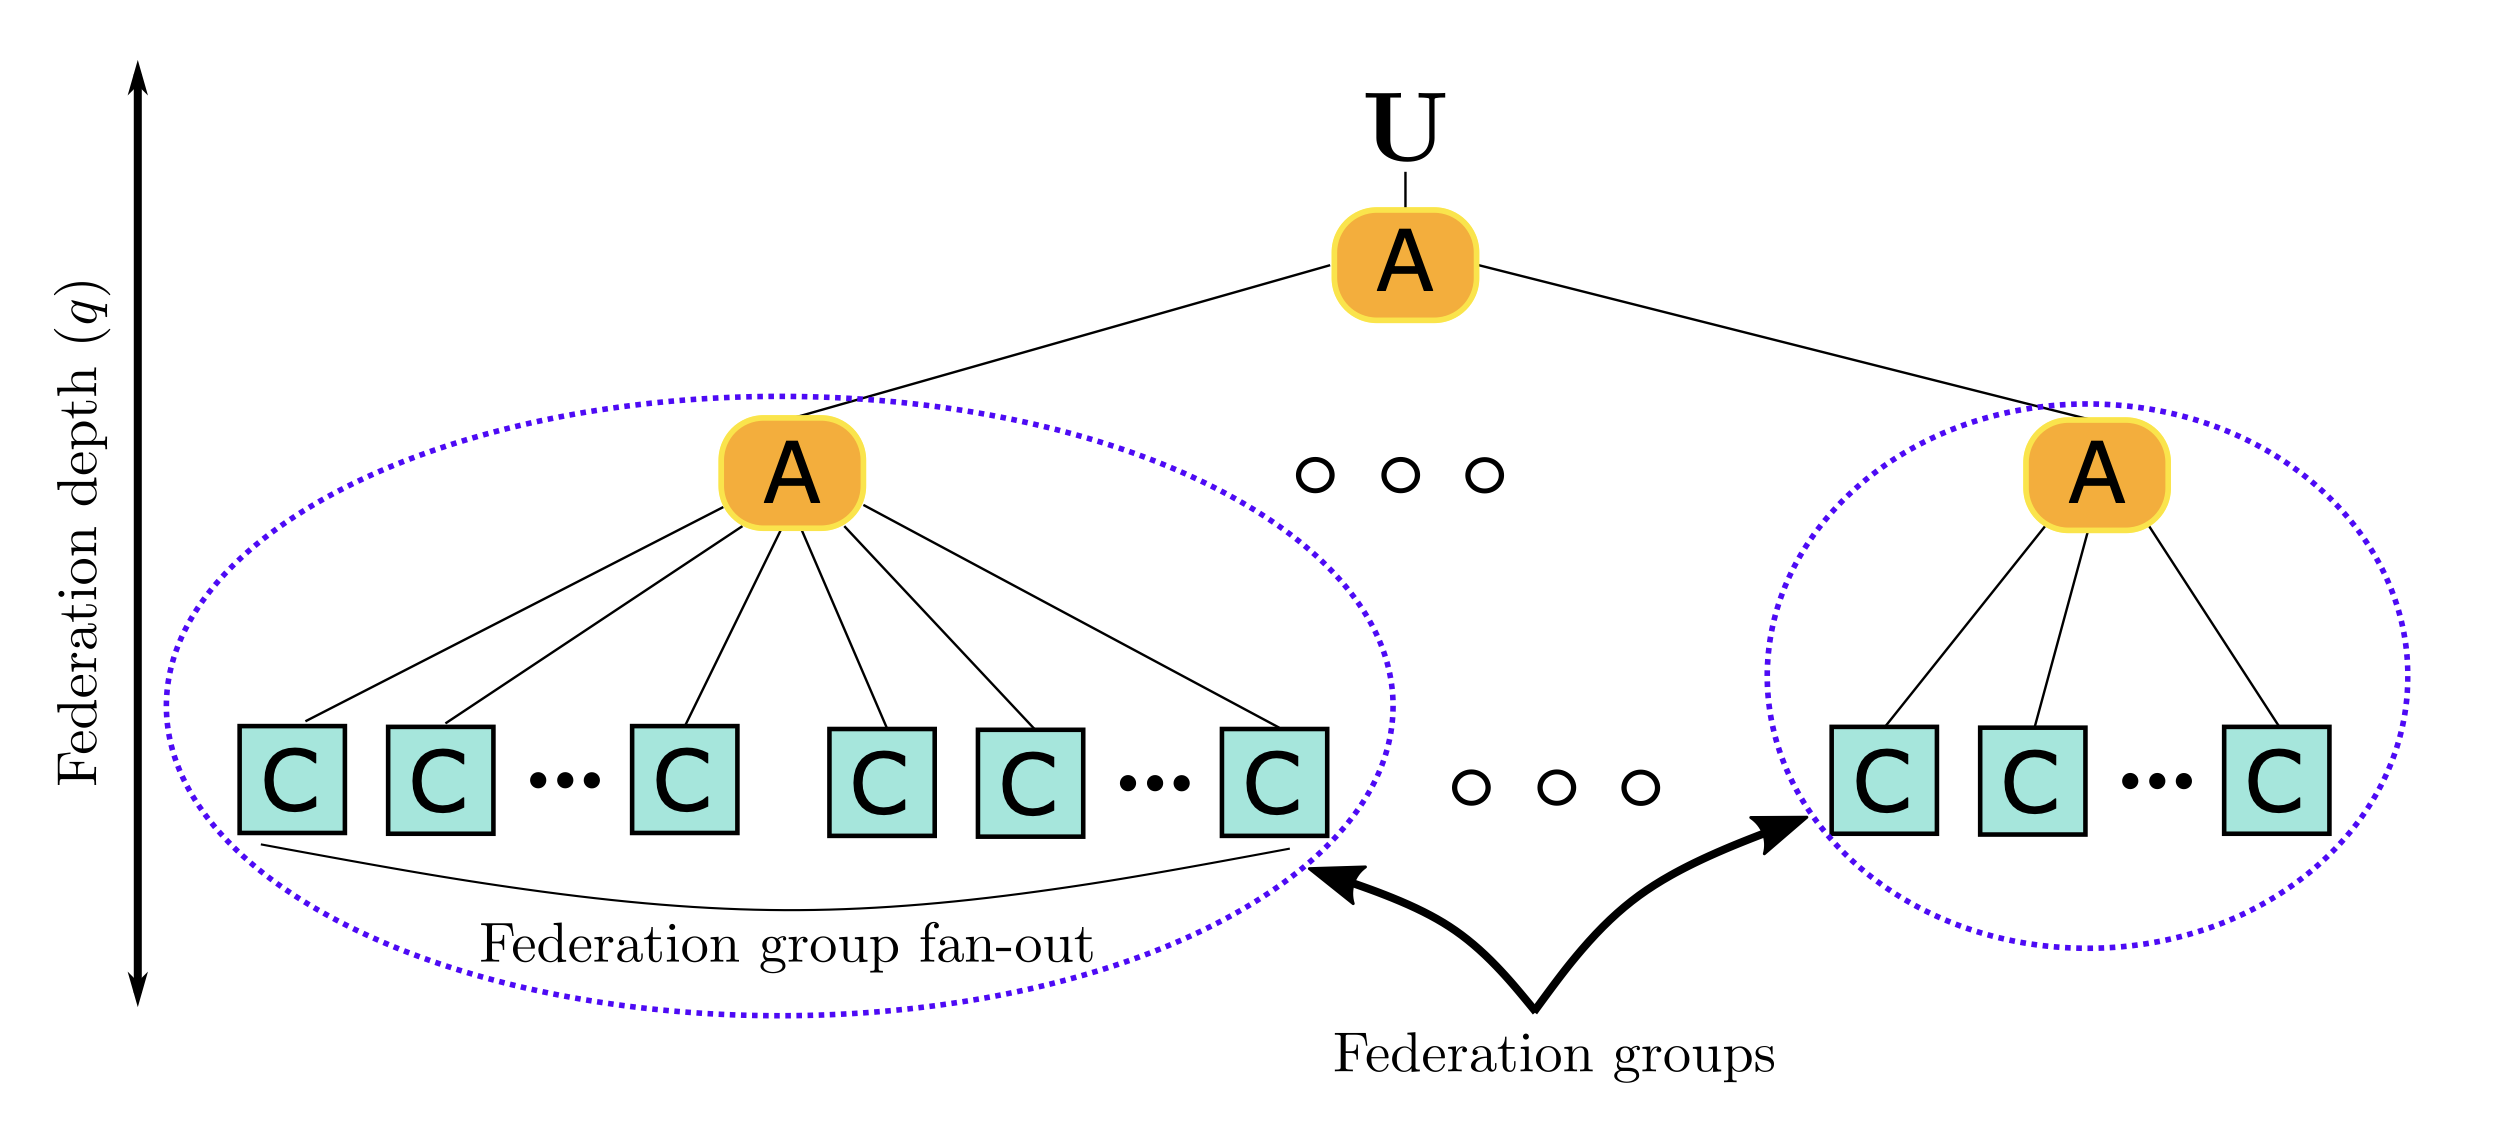
\includegraphics[width=\textwidth]{images/pronto-agg.png}
    \caption{How local models are aggregated in \textsc{Pronto}. Dedicated aggregator
    Nodes propagate the updated subspaces until the root is reached.}
    \label{pronto-agg}
\end{figure}
\textsc{Pronto} aggregation resembles the distributed agglomerative summary
model (DASM) \cite{}. Local models are aggregated in a "bottom-up" approach
following a tree-structure depicted in Figure \ref{pronto-agg}. While this
approach reportedly requires minimal synchonisation, it demands
multiple dedicated Pods, and Kubernetes' inherent communication latency could
significantly delay global model updates after workload changes.

Therefore, I opted for a ``flat" on-the-fly aggregation approach: when the
Aggregation Server receives an aggregation request with a Node's local model,
instead of aggregating the local model and returning the new global model, the
server first enqueues the local model to be aggregated and returns its current
view of the global model. This implementation trades consistency for latency.

\begin{figure}[H]
    \centering
    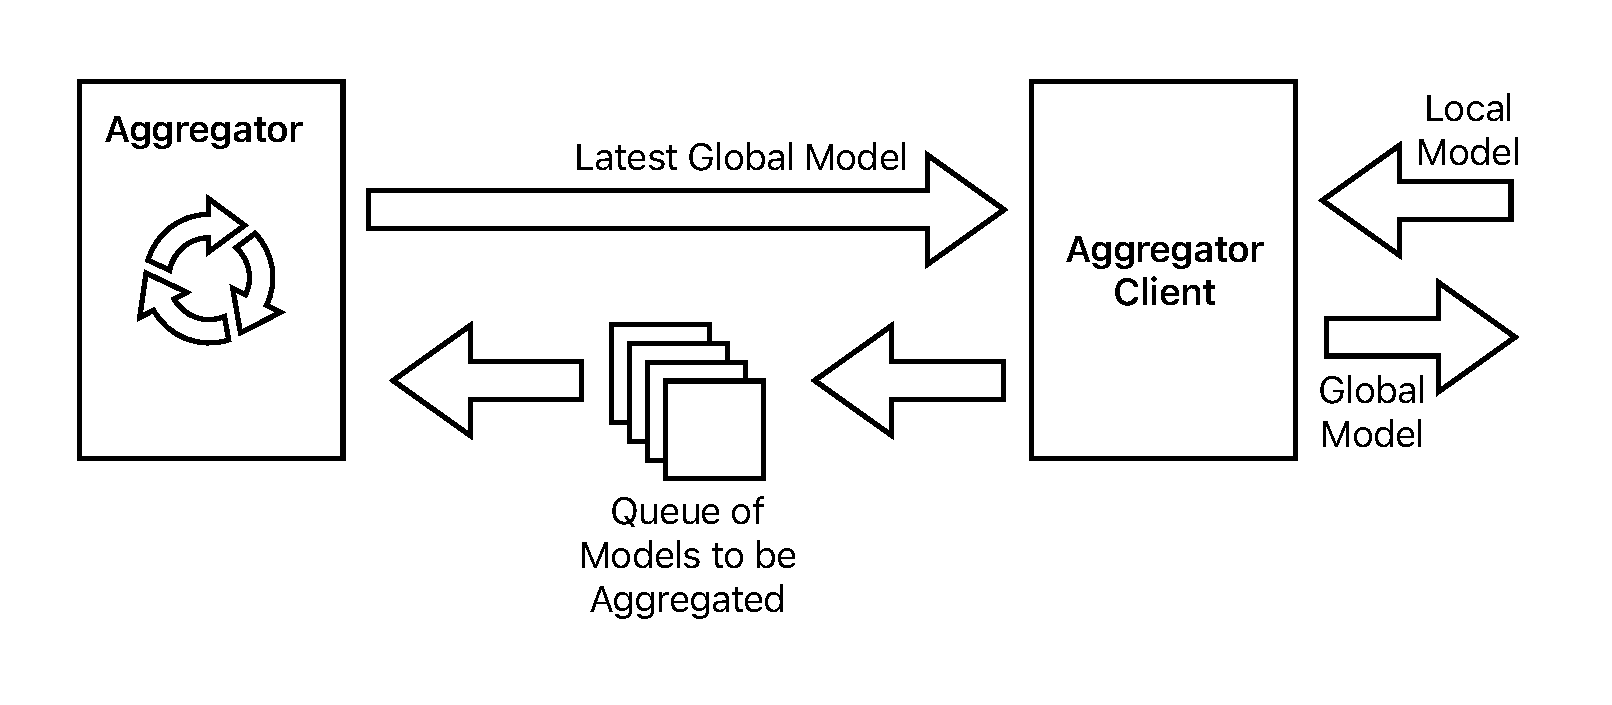
\includegraphics[width=\textwidth]{images/spazio-agg.pdf}
    \caption{The components within the Aggregator Server.}
    \label{spazio-agg-components}
\end{figure}

The Aggregation Server executes a thread which waits on a queue of local models
to aggregate. When the queue is non-empty, the thread pops the local model and
performs a Subspace Merge operation (as defined in \ref{sec:local-merge}). To
balance the influence of each local model, weights $\gamma_{\mathbf{A}} =
\text{\# of Nodes} - 1$ and $\gamma_{\mathbf{B}} = 1$ are used in the
Subspace-Merge (as per Section \ref{sec:local-merge}).
Aggregation clients perform a gRPC call to the address specified by the
Aggregation Service. This gRPC function is implemented by the server and takes
the local model of a Node as its argument. The function first enqueues the local
model to be merged and returns the latest view of the global model. Clients
then aggregate their own local model with the received global model. Decoupling
model aggregation from the gRPC call's critical path reduces server load,
improving its capacity to handle more clients.

\section{Scheduler Pod}
\subsection{Kubernetes Scheduler Plugin}
\begin{figure}[H]
    \centering
    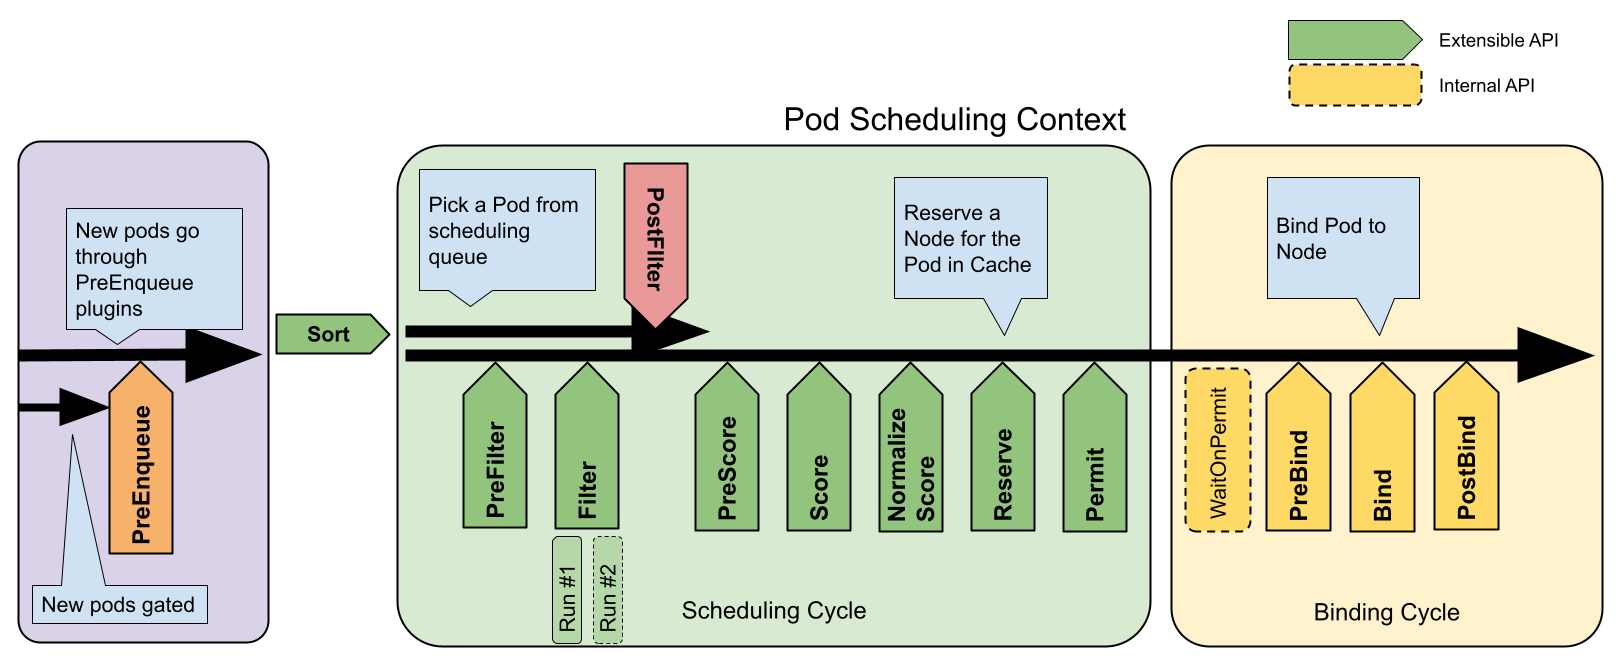
\includegraphics[width=\textwidth]{images/scheduling-framework-extensions.png}
    \caption{The available scheduling framework extension points
    \cite{scheduling-framework}.}
    \label{fig:kube-sched-framework}
\end{figure}
The scheduling framework (depicted in Figure \ref{fig:kube-sched-framework}) is
a pluggable architecture for the Kubernetes scheduler. It defines extension
points at which scheduler plugins register to be invoked. A scheduler plugin can
register to multiple extension points, with each extension point defining an
interface: a set of functions the scheduler plugin has to implement.

Developing a \textsc{Carico}-based scheduler plugin, rather than a standalone
scheduelr, simplified implemention and offered many performance benefits. First,
\textsc{Carico}'s scheduling operations (Section \ref{sec:spazio-cost-capacity}
map well to the framework's extension points. Second, the framework provides
access to efficient, pre-existing data structures and algorithms. Finally,
plugins allow customisation through selective enabling/disabling of default
plugins and ordering of custom ones. This means that the \textsc{Carico} plugin
could be used in tandem with other plugins to improve scheduling decisions.

The \textsc{Carico} scheduler tracks Pod reservations using a \verb|map| (Pod ID
to Node ID) and a Kubernetes API Pod Event Listener. During the Reserve phase, the scheduler
increments the target Node's reserve count and records Pod-Node assignment. When
the API listener detects a Pod transitioning from the 'Pending'
status, if the Pod is in its reservation \verb|map|, the scheduler decrements
the corresponding Node's reserved count.
